Frequentist estimators are those most often encountered in undergraduate studies including basic statistics. The term frequentist hints at the estimators utilizing the frequency with which observations appear to estimate underlying models. Extremum estimation is a generalized framework to study these estimators. Common for all extremum estimators is a \textit{stochastic criterion function} $Q_N(\theta)$ which is to be minimized, as well as data $w_i = \{y_i, x_i'\}_{i = 1}^N$. Using these ingredients, as well as a set of assumptions (i.e. $E[\epsilon|x] = 0$) and a parametric representation of the model. An extremum estimator is formally then an estimator which solves
\begin{equation}
\hat{\theta}_{E} = \underset{\theta}{\textrm{arg min }}  Q_N(\theta)
\end{equation}

In these notes all of the frequentist estimators studied will be asymptotically normal, with limit distribution (more on this later)
\begin{equation}
\hat{\theta}_N \overset{a}{\sim} \mathcal{N}(\theta_0, A_0^{-1}B_0 A_0^{-1})
\end{equation}

Usually the two matrices $A_0$ and $B_0$ can be estimated by the hessian and the outer product of the gradients respectively. It is the criterion function $Q_N(\cdot)$ that essentially defines the properties of an estimator. A subgroup of extremum estimators is the M estimators, defined by solving the problem
\begin{equation}
\hat{\theta}_N = \underset{\theta}{\textrm{arg min }} \frac{1}{N} \sum_{i=1}^N q(w_i, \theta)
\end{equation}
In other words M-estimators are extremum estimators where $Q_N(\theta) = \frac{1}{N} \sum_{i=1}^N q(w_i , \theta)$. The advantage to working with M-estimators compared to the more general extremum estimators, is that they allow for the application of a law of large number and the central limits theorem.
\subsection{Identification}
Identification essentially ensures that one can estimate a unique solution for each of the model parameters. Mathematically $\theta_1$ is identified if $P_{\theta_1}(w) = P_{\theta_2}(w), \forall w \in \mathcal{W}$ iff $\theta_1 = \theta_2$. In the case of extremum estimators this is equivalent with the requirement that
\begin{equation}
Q(\theta_0) < Q(\theta), \quad \forall \theta \in \Theta : \theta \neq \theta_0
\end{equation}
In the case of M-estimators this can be reduced to
\begin{equation*}
E[q(w_i,\theta_0)] < E[q(w_i, \theta)], \quad \forall \theta \in \Theta : \theta \neq \theta_0
\end{equation*}

\subsection{Consistency}
Assuming the specified model is correct compared to the underlying datagenerating process (DGP), and thus is identified we can derive consistency on the basis of the criterion function. Consistency is the notion that for large values of the sample size $N$ the estimator should converge in probability to $\theta_0$, formally a convergent estimator $\hat{\theta}_N$ has the property that
\begin{equation}
\textrm{plim } \hat{\theta}_N = \theta_0
\end{equation}
or equivalently
\begin{equation}
\lim_{N \rightarrow \infty} \textrm{Pr}\left(
 |\hat{\theta}_N - \theta_0|> \epsilon
\right)
= 0, \quad \forall \epsilon > 0
\end{equation}
In simple cases, such as for OLS we know how to express the model in simple terms that allow for the derivation of consistency, but in the general case we know nothing else than the criterion function $Q_N(\cdot)$. The concept is illustrated in figure \ref{fig: consistentextremum}.

\begin{figure}
\caption{Concept of consistency in extremum estimators}
\label{fig: consistentextremum}
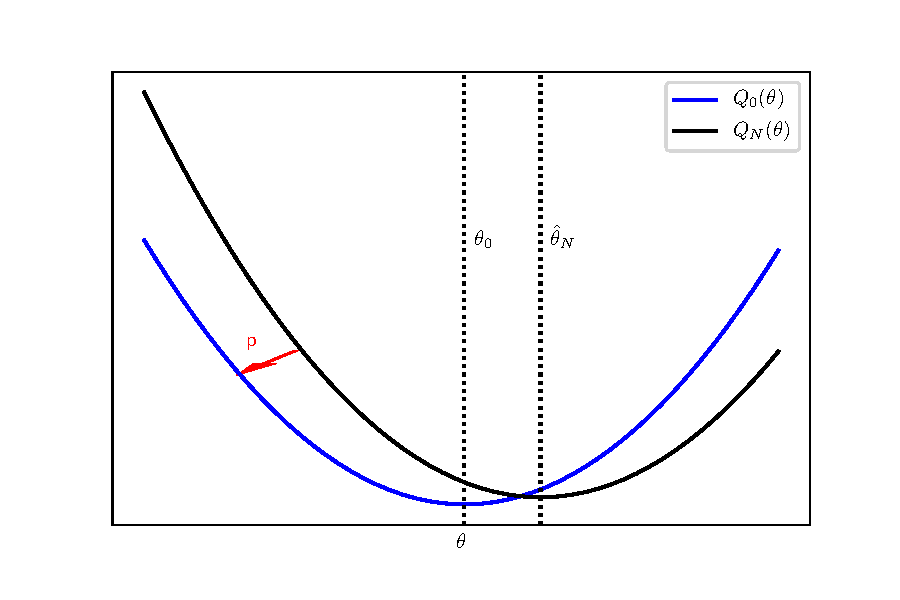
\includegraphics[width = \linewidth]{figures/extremumconv}
\caption*{As $N$ increases consistency will mean for the criterion function $Q_N(\theta)$ to converge in probability to the actual criterion function $Q_0(\theta)$, thus yielding a consistent estimate of $\hat{\theta}_N$.}
\end{figure}

We can think of $Q_N(\cdot)$ as the sample criterion function, which when minimized yields a sample parameter estimate $\hat{\theta}_0$, and likelise the population criterion $Q_0(\cdot)$ yields the true parameter $\theta_0$. The goal in showing consistency is to show that the sample criterion converges in probability to $Q_0(\cdot)$. For M-estimators applying a law of large numbers gives that
\begin{equation}
\frac{1}{N} \sum_{i=1}^N q(w_i, \theta) \underset{N \rightarrow \infty}{\rightarrow} E[q(w_i, \theta)] \equiv Q_0(\theta)
\end{equation}
but this is not possible in the case of extremum estimators. Instead, c.f theorem 5.1 of C\&T the following assumptions will ensure that an estimator $\hat{\theta}_N$ is consistent:
\begin{itemize}
\item The parameter space $\Theta$ is a compact subset of $\mathbb{R}^q$, compact meaning closed an bounded. (Note that $\mathbb{R}$ is not compact, making this asusmptions untrue for most estimation methods in practise).
\item $Q_N(\theta)$ is measurable and continous for all $\theta \in \Theta$.
\item $Q_N(\theta)$ converges uniformly in probability to a nonstochastic function $Q_0(\theta)$, which has a unique global maximum at $\theta_0$.
\end{itemize}
Assuming continuity and measurability of $Q_N(\theta)$ and compactness of $\Theta$ allows to invoke the extreme value theorem, which simply guarantees that a minimum and amaximum of $Q_N(\cdot)$ over a closed interval $[a,b]$ will exist.

\subsection{Asymptotic distribution}
To derive the limit distribution of $\hat{\theta}_N$ we will invoke the \textit{mean value theorem}, which has a very intuitive graphical presentation shown in figure \ref{fig: MVT}. Mathematically we simply equate the derivative of a function, measured in a point $x^+$ with the slope of a line connecting two points $[x_0,x_1]$. To use the theorem it is required that $Q_N(\cdot)$ is twice differentiable around $\theta_0$. Applying the mean value theorem on $\frac{\partial Q_N(\theta)}{\partial \theta}$ on the interval $[\hat{\theta}_N, \theta_0]$ will yield

\begin{multline}
\frac{\partial Q_N(\theta)}{\partial \theta} \bigg{|}_{\hat{\theta}_N} =
\frac{\partial Q_N(\theta)}{\partial \theta} \bigg{|}_{\theta_0} \\ +
\frac{\partial^2 Q_N(\theta)}{\partial \theta \partial \theta'} \bigg{|}_{\theta^+}(\hat{\theta}_N - \theta_0)
\end{multline}

Where by definition $\frac{\partial Q_N(\theta)}{\partial \theta} \bigg{|}_{\hat{\theta}_N} = 0$ so rearranging leaves us with


\begin{multline} \label{eq: asyms}
\sqrt{N}(\hat{\theta}_N - \theta_0) = \left( \frac{\partial^2 Q_N(\theta)}{\partial \theta \partial \theta'} \bigg{|}_{\theta^+} \right)^{-1}  \\ \times
\left(
\frac{\partial Q_N(\theta)}{\partial \theta} \bigg{|}_{\theta_0} \sqrt{N}
\right)
\end{multline}


\begin{figure}
\caption{Mean Value Theorem illustration}
\label{fig: MVT}
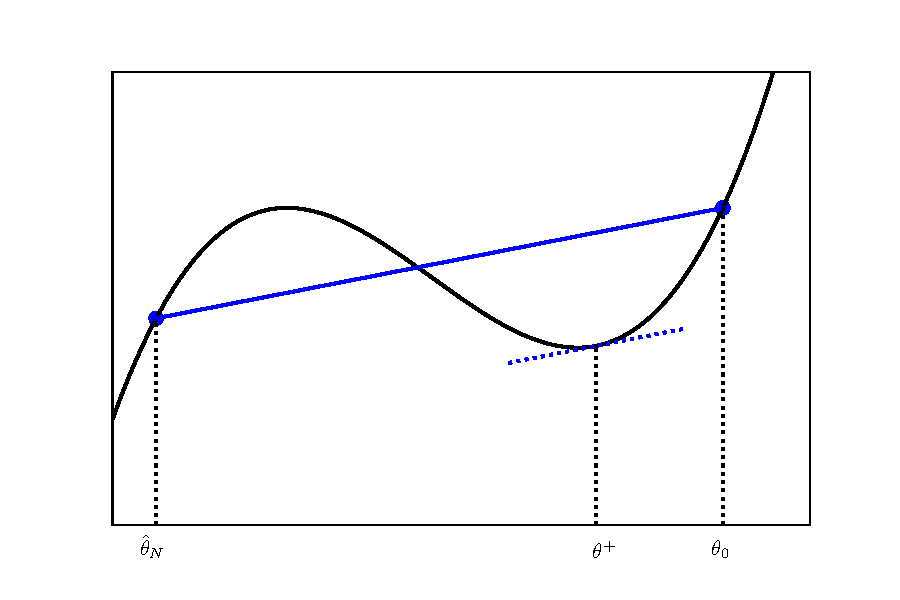
\includegraphics[width = \linewidth]{figures/mvt}
\caption*{The mean value theorem essentially tells us that any continous function $f(z)$ over the interval $\mathcal{I}$ will have at least one point in $\mathcal{I}$ where $\frac{\partial f(z)}{\partial z}$ equals the slope between the endpoints of $\mathcal{I}$.}
\end{figure}

It is then assumed that the following matrices exist and, that the terms converge towards
\begin{align*}
&\frac{\partial^2 Q_N(\theta)}{\partial \theta \partial \theta'} \bigg{|}_{\theta^+} \overset{p}{\rightarrow} A_0 \\
& \frac{\partial Q_N(\theta)}{\partial \theta} \bigg{|}_{\theta_0} \sqrt{N} \overset{d}{\rightarrow} \mathcal{N}(0,B_0)
\end{align*}
If $A_0$ and $B_0$ exist, we can then see from the expression in \eqref{eq: asyms} that asymptotically a consistent M estimator $\hat{\theta}_N$ has distribution
 \begin{equation}
 \sqrt{N}(\hat{\theta}_N - \theta_0) \overset{d}{\rightarrow} \mathcal{N}(0, A_0^{-1}B_0A_0^{-1})
 \end{equation}
In practise of course $A_0$ and $B_0$ are unknown, and will have to be estimated, usually with the following empirical matrices

\begin{align*}
&\hat{A} = \frac{\partial^2 Q_N(\theta)}{\partial \theta \partial \theta'} \bigg{|}_{\hat{\theta}}
\\
& \hat{B} = \frac{1}{N} \sum_{i=1}^N \frac{\partial q(w_i, \theta)}{\partial \theta} \bigg{|}_{\hat{\theta}} \frac{\partial q(w_i, \theta)}{\partial \theta'} \bigg{|}_{\hat{\theta}}
\end{align*}

\subsubsection{Maximum likelihood estimators}
Maximum likelihood estimators has the property that $Q_N(\theta)$ is specified so that
\begin{equation}
Q_N(\theta) = - \sum_{i=1}^N \log L_i(\theta| x_i,y_i)
\end{equation}
Because of this the sandwich expression for the variance derived above collapses to an even simpler expression where $\hat{\theta}_{ML} \sim \mathcal{N}(0, [\mathcal{I}(\theta)]^{-1})$ where $\mathcal{I}(\theta)$ is the fischer information, defined as
\begin{equation}
\mathcal{I}(\theta) = -E\left[ \frac{\partial^2 \log L_i(\theta| x_i,y_i)}{\partial \theta \partial \theta'} \right]
\end{equation}
The proof of this is as follows

Use that $\log L_i(\theta |x_i, y_i) \propto f(y_i | \theta)$, that is the likelihood is proportional to the density of the data. Starting here, we know that
\begin{equation}
\int_{\mathbb{R}} f(y_i | \theta) = 1
\end{equation}
and since the bound of the integral does not depend on $\theta$ taking the derivative w.r.t it on both sides gives
\begin{equation}
\int_{\mathbb{R}} \frac{\partial}{\partial \theta} f(y_i | \theta) = 0
\end{equation}
Now apply that $\frac{\partial \log f(x)}{\partial x} = \frac{\partial f(x)}{\partial x} [f(x)]^{-1}$ to get
\begin{equation}
\int_{\mathbb{R}} \frac{\partial \log f(y_i | \theta)}{\partial \theta}  f(y_i | \theta) = 0
\end{equation}
Using again the rewrite of the derivative of the log of a function gives
\begin{align}
&\int_{\mathbb{R}} \frac{\partial}{\partial \theta} \frac{\partial \log f(y_i | \theta)}{\partial \theta}  f(y_i | \theta) = 0
\end{align}
Which when written out gives
\begin{align*}
 \int_{\mathbb{R}}  &\frac{\partial \log f(y_i | \theta)}{\partial \theta}  \frac{\partial f(y_i | \theta)}{\partial \theta}
\\ &+ \frac{\partial^2 \log f(y_i | \theta)}{\partial \theta \partial \theta'} f(y_i|\theta)
 = 0
\end{align*}
Using the log-derivative trick one final time gives the desired result
\begin{align*}
 \int_{\mathbb{R}}  &\frac{\partial f(y_i | \theta)}{\partial \theta}  \frac{\partial f(y_i | \theta)}{\partial \theta} f(y_i | \theta)
\\ &+ \frac{\partial^2 \log f(y_i | \theta)}{\partial \theta \partial \theta'} f(y_i|\theta)
 = 0
\end{align*}
Or written in terms of expectations
\begin{equation}
E \left[
\frac{\partial f(y_i | \theta)}{\partial \theta}  \frac{\partial f(y_i | \theta)}{\partial \theta}
\right]
= - E\left[
\frac{\partial^2 \log f(y_i | \theta)}{\partial \theta \partial \theta'}
\right]
\end{equation}
Comparing this expression to the $A_0^{-1}B_0A_0^{-1}$ expression derived above should make it clear why the asymptotic variance of maximum likelihood estimators simplifies to the fischer information.
